\documentclass[12pt,a4paper]{article}
\usepackage[utf8]{inputenc}
\usepackage[T1]{fontenc}
\usepackage{graphicx}
\usepackage[table,dvipsnames]{xcolor}
\usepackage{hyperref}
\usepackage{enumitem}
\usepackage{titlesec}
\usepackage{geometry}
\usepackage{booktabs}
\usepackage{array}
\usepackage{multirow}
\usepackage{tikz}
\usepackage{amssymb}
\usepackage{rotating}
\usepackage{adjustbox}
\usepackage{pdflscape}
\usepackage{longtable}
\usepackage{float}
\usepackage{colortbl}
\usepackage{tcolorbox}
\usepackage{caption}
\usepackage{setspace}
\usepackage{fancyhdr}
\tcbuselibrary{skins}
\usetikzlibrary{shapes,arrows,positioning,fit,backgrounds}
\usepackage{tabularx} % For dynamic table widths

% Page layout
\geometry{a4paper, margin=2.5cm, headheight=15pt}
\setlength{\parindent}{0pt}
\setlength{\parskip}{6pt}

% Improve table formatting
\renewcommand{\arraystretch}{1.2}

% Header and footer setup
\pagestyle{fancy}
\fancyhf{}
\renewcommand{\headrulewidth}{0.4pt}
\renewcommand{\footrulewidth}{0.4pt}
\fancyhead[L]{IFPE - Chatbot com IA}
\fancyhead[R]{Plano de Implantação}
\fancyfoot[C]{\thepage}

% Redefine clear double page to avoid blank pages if needed
\let\cleardoublepage\clearpage

% Section formatting
\titleformat{\section}
  {\normalfont\Large\bfseries\color{blue!80!black}}{\thesection}{1em}{}
\titleformat{\subsection}
  {\normalfont\large\bfseries\color{blue!60!black}}{\thesubsection}{1em}{}
\titleformat{\subsubsection}
  {\normalfont\normalsize\bfseries\color{blue!40!black}}{\thesubsubsection}{1em}{}
  
% Float placement preferences
\renewcommand{\topfraction}{0.85}
\renewcommand{\bottomfraction}{0.85}
\renewcommand{\textfraction}{0.1}
\renewcommand{\floatpagefraction}{0.75}

% Better caption styling
\captionsetup{font=small,labelfont=bf,justification=centering,margin=1cm}

\hypersetup{
    colorlinks=true,
    linkcolor=blue,
    filecolor=magenta,      
    urlcolor=cyan,
    pdftitle={Plano de Implantação - Chatbot com IA para Processos de Segurança do Trabalho IFPE},
    pdfauthor={Pedro Balbino, Eric Barreto, Lucas Lucena, Sara Pereira, Luis Felipe Guedes},
}

\begin{document}

\begin{titlepage}
    \thispagestyle{empty}
    \centering
    \vspace*{0.5cm}
    % Uncomment the line below when you have the actual logo file
    {\includegraphics[width=4cm]{images/UFPE.jpg}\par}
    \vspace{1cm}
    {\scshape\LARGE Instituto Federal de Pernambuco \par}
    \vspace{1.5cm}
    {\huge\bfseries Plano de Implantação \par}
    \vspace{1cm}
    {\Large\itshape Chatbot com IA para Processos de Segurança do Trabalho\par}
    \vfill
    \begin{center}
    \begin{tabular}{c}
        {\large \textbf{Elaborado por:}}\\[0.5cm]
        Pedro Henrique Souza Balbino\\
        Eric Bezerra Londres Barreto\\
        Lucas Lucena Xavier de Morais\\
        Sara Simone Emilay de Araujo Pereira\\
        Luis Felipe Guedes Souto Moreira\\
        Maria Beatriz Martins Pontes Gonçalo\\
        Pablo Henrique Ferreira da Silva\\
        Vinicius Nobre da Silva Prazeres
    \end{tabular}
    \end{center}
    \vfill
    {\large Abril de 2025\par}
\end{titlepage}

\newpage
\thispagestyle{empty}
\section*{Histórico de Revisões}

\begin{table}[h]
\centering
\renewcommand{\arraystretch}{1.3}
\begin{tabular}{|c|c|p{8cm}|c|}
\hline
\rowcolor{gray!15}\textbf{Revisão} & \textbf{Data} & \textbf{Descrição} & \textbf{Autor} \\
\hline
1 & 25/03/2025 & Versão inicial do documento & Pedro Balbino \\
\hline
2 & 01/04/2025 & Revisão com incorporação de feedback do cliente & Eric Barreto \\
\hline
3 & 05/04/2025 & Versão final para apresentação & Equipe do Projeto \\
\hline
\end{tabular}
\end{table}

\clearpage
\tableofcontents
\thispagestyle{empty}
\clearpage

\section{Introdução}

\subsection{A Organização}
O Instituto Federal de Educação, Ciência e Tecnologia de Pernambuco (IFPE) é uma instituição de ensino superior pública federal vinculada ao Ministério da Educação. Fundado em 2008 a partir da integração do Centro Federal de Educação Tecnológica de Pernambuco (CEFET-PE) e das Escolas Agrotécnicas Federais, o IFPE atualmente possui 16 campi distribuídos por todo o estado de Pernambuco, oferecendo educação profissional, científica e tecnológica de qualidade, em diferentes modalidades e níveis de ensino.

Com aproximadamente 18.000 alunos e 2.500 servidores (docentes e técnicos administrativos), o IFPE tem como missão promover a educação profissional, científica e tecnológica, em todos os seus níveis e modalidades, com base no princípio da indissociabilidade das ações de Ensino, Pesquisa e Extensão, comprometida com uma prática cidadã e inclusiva, de modo a contribuir para a formação integral do ser humano e para o desenvolvimento sustentável da sociedade.

\subsection{O projeto e seu propósito}
O projeto consiste na implementação de um chatbot com Inteligência Artificial destinado a automatizar processos de segurança do trabalho no IFPE. O propósito principal é melhorar a comunicação e a gestão dos processos relacionados à área de segurança do trabalho, fornecendo uma plataforma unificada que centralize informações, automatize o preenchimento de formulários e oriente os usuários durante solicitações relacionadas à segurança do trabalho.

Os objetivos específicos do projeto incluem:

\begin{itemize}
    \item Centralizar a documentação técnica de segurança do trabalho em um repositório de fácil acesso
    \item Automatizar o preenchimento de formulários para reduzir erros e retrabalho
    \item Padronizar os processos de solicitação relacionados à segurança do trabalho
    \item Diminuir a carga de trabalho administrativo da equipe técnica do SIASS
    \item Melhorar a experiência dos servidores ao interagir com o setor de segurança do trabalho
    \item Garantir o cumprimento de normas e procedimentos de segurança
\end{itemize}

\subsection{Equipe do projeto}
A equipe responsável pela elaboração deste plano de implantação e pela condução do projeto é composta por:

\begin{table}[h]
\centering
\begin{tabular}{|p{5cm}|p{8cm}|}
\hline
\textbf{Nome} & \textbf{Função no Projeto} \\
\hline
Pedro Henrique Souza Balbino & Gerente de Projeto / Analista de Processos \\
\hline
Eric Bezerra Londres Barreto & Arquiteto de Soluções / Especialista em IA \\
\hline
Lucas Lucena Xavier de Morais & Desenvolvedor / Integração de Sistemas \\
\hline
\hline
Luis Felipe Guedes Souto Moreira & Desenvolvedor / Engenheiro de Dados \\
\hline
Maria Beatriz Martins Pontes Gonçalo & Designer de UX/UI \\
\hline
Pablo Henrique Ferreira da Silva & Especialista em Segurança da Informação \\
\hline
Vinicius Nobre da Silva Prazeres & Analista de Qualidade / Testes \\
\hline
\end{tabular}
\end{table}

\pagebreak

\begin{itemize}
    \item Mauro César de Oliveira (Especialista em Segurança do Trabalho - SIASS/IFPE)
    \item Marco Antônio Eugênio Araujo (Representante SIASS/Cliente)
    \item Equipe do Núcleo de Tecnologia da Informação (NTI) do IFPE
\end{itemize}

\section{Contexto da unidade em estudo}

\subsection{Histórico da unidade de negócio}
O Subsistema Integrado de Atenção à Saúde do Servidor (SIASS) foi instituído pelo Decreto nº 6.833, de 29 de abril de 2009, como parte da Política de Atenção à Saúde e Segurança do Trabalho do Servidor Público Federal (PASS). Sua principal função é coordenar e integrar ações e programas nas áreas de assistência à saúde, perícia oficial, promoção, prevenção e acompanhamento da saúde dos servidores da administração federal.

No IFPE, a unidade SIASS atende não apenas aos servidores da própria instituição, mas também a diversos órgãos públicos federais da região, conforme evidenciado na ata de reunião de 06 de fevereiro de 2025: \textit{"O SIASS atende vários órgãos públicos federais para otimizar recurso financeiro orçamentário. É um órgão dividido compartilhado por vários órgãos e ele está no IFPE, mas atende vários órgãos públicos, dentre eles o próprio IFPE mais polícia rodoviária."} 

O setor de Segurança do Trabalho, foco deste projeto, é um dos componentes do SIASS e tem como responsabilidade garantir condições seguras e saudáveis no ambiente de trabalho, através de avaliações de risco, emissão de laudos técnicos, treinamentos e orientações aos servidores.

\subsection{Principais stakeholders}
Os principais stakeholders envolvidos no escopo do projeto são:

\begin{table}[h]
\centering
\begin{tcolorbox}[enhanced, colback=white, colframe=gray!40, arc=4mm, boxrule=1pt]
\begin{tabular}{p{4cm}p{10cm}}
\textbf{Stakeholder} & \textbf{Papel no Projeto} \\
\hline
\textbf{Equipe técnica de Segurança do Trabalho do SIASS} & Responsável pela avaliação de ambientes laboratoriais, emissão de laudos técnicos, gestão de EPIs e análise de riscos ocupacionais. São os usuários primários da plataforma em seu papel administrativo. \\
\hline
\textbf{Servidores do IFPE} & Docentes, técnicos administrativos e outros colaboradores que necessitam interagir com o setor de segurança do trabalho para solicitar avaliações, relatórios, documentos ou orientações. \\
\hline
\textbf{Funcionários terceirizados} & Prestadores de serviço que atuam nas instalações do IFPE e que também estão sujeitos às normas de segurança do trabalho. \\
\hline
\textbf{Gestores departamentais} & Responsáveis pela aprovação e acompanhamento de solicitações relacionadas à segurança do trabalho em suas respectivas áreas. \\
\hline
\textbf{Núcleo de Tecnologia da Informação (NTI)} & Área responsável pela infraestrutura tecnológica do IFPE e pelo suporte técnico à solução a ser implementada. \\
\hline
\textbf{Alta administração do IFPE} & Reitoria e pró-reitorias que definem diretrizes e políticas institucionais, além de aprovar recursos para projetos estratégicos. \\
\end{tabular}
\end{tcolorbox}
\caption{Mapeamento de Stakeholders do Projeto}
\end{table}

\subsection{Objetivos da unidade de negócio}
Os objetivos do setor de Segurança do Trabalho do SIASS/IFPE incluem:

\begin{itemize}
    \item Garantir a saúde e segurança dos servidores no ambiente de trabalho
    \item Prevenir acidentes e doenças ocupacionais através de medidas preventivas
    \item Assegurar o cumprimento das normas regulamentadoras e legislação de segurança do trabalho
    \item Realizar avaliações de ambientes e emitir laudos técnicos
    \item Desenvolver e implementar programas de prevenção de riscos ambientais
    \item Proporcionar treinamentos e orientações sobre segurança do trabalho
    \item Investigar e analisar acidentes de trabalho
    \item Gerenciar a concessão de adicionais ocupacionais
    \item Fornecer documentação necessária para processos de aposentadoria especial
\end{itemize}

O setor enfrenta desafios significativos devido à equipe reduzida e à alta demanda de serviços, conforme destacado na reunião de 06 de fevereiro de 2025: \textit{"A equipe de César é pequena e ele tem muita demanda então acaba que esse tratamento Inicial [...] é um problema."}

\subsection{Sistema/solução atualmente implantado(a)}
Atualmente, o setor de Segurança do Trabalho do SIASS utiliza uma combinação de sistemas e processos manuais para gerenciar suas atividades:

\begin{itemize}
    \item \textbf{Sistema Eletrônico de Informação (SEI):} Utilizado para a tramitação de processos e documentos oficiais. Conforme mencionado na ata de reunião de 11 de março de 2025, o SEI é o \textit{"principal sistema utilizado atualmente para trâmite de processos e documentos oficiais no IFPE."} No entanto, o sistema não foi concebido especificamente para a gestão de segurança do trabalho e apresenta limitações para este fim.
    
    \item \textbf{SEAPNET:} Sistema do Governo Federal para registro de acidentes de trabalho, com dados desde 2009, conforme mencionado na ata de reunião de 25 de março de 2025.
    
    \item \textbf{Planilhas e documentos locais:} Grande parte das informações é gerenciada através de documentos Microsoft Word e planilhas Excel armazenadas localmente, sem um sistema centralizado.
    
    \item \textbf{E-mail e telefone:} A comunicação com os solicitantes e entre departamentos é frequentemente realizada por e-mail ou telefone, sem padronização ou registro sistemático.
    
    \item \textbf{Formulários físicos:} Diversos processos ainda utilizam formulários em papel que precisam ser preenchidos manualmente.
    
    \item \textbf{Site institucional:} Uma seção do site do IFPE é utilizada para disponibilizar alguns documentos relacionados à segurança do trabalho, mas com limitações quanto à atualização e facilidade de acesso.
\end{itemize}

O especialista em segurança do trabalho, Sr. César, relatou que o sistema SEI é inadequado para a gestão de documentos de segurança, pois \textit{"é voltado para processos que têm início e fim, enquanto documentos de segurança são contínuos e precisam ser constantemente atualizados"} (Ata de reunião de 25 de março de 2025).

\newpage
\section{Análise de estados}

\subsection{Estado Atual}

\subsubsection{Escopo do processo}
O escopo atual dos processos de segurança do trabalho no IFPE engloba uma série de atividades essenciais para garantir a saúde e segurança dos servidores. Com base no documento "Mapeamento de Processos de Segurança aplicáveis ao IFPE" e nas atas de reunião, foram identificados os seguintes macroprocessos:

\begin{itemize}
    \item Gestão de Acidentes do Trabalho
    \item Gestão de Mapeamento e Graduação de Riscos
    \item Gestão de Equipamentos de Proteção Individual (EPIs)
    \item Gestão de Treinamento de SST
    \item Gestão do Plano de Emergência
    \item Gestão de Energias Perigosas
    \item Gestão de Auditorias e Inspeções de Segurança
    \item Gestão de Critérios Mínimos para Contratação de Empresas Terceirizadas
    \item Gestão de Mudanças
    \item Gestão de Documentos de SST
    \item Gestão de Uso de Produtos Químicos
    \item Gestão de Projetos de Novas Instalações com foco em SST
    \item Gestão de concessão de adicionais ocupacionais
    \item Gestão de documentos de aposentadoria especial (PPP)
\end{itemize}

Cada um desses macroprocessos é composto por diversos subprocessos e atividades, que atualmente são executados de forma fragmentada e com baixo grau de automação.

\subsubsection{Processos - As Is (Modelagem dos processos atualmente implementados)}

O fluxo de trabalho atual do setor de Segurança do Trabalho no IFPE segue uma abordagem predominantemente manual e fragmentada, conforme detalhado nas atas de reunião. A seguir, apresentamos a modelagem do processo genérico que representa a maior parte das solicitações:

\clearpage
\begin{landscape}
\thispagestyle{fancy}
\begin{figure}[H]
\makebox[\linewidth][c]{
\includegraphics[width=0.98\paperwidth, height=0.9\paperheight, keepaspectratio]{images/AS-IS.jpg}
}
\caption{Processo Atual (As-Is) de Solicitação de Segurança do Trabalho}
\end{figure}
\end{landscape}
\clearpage

Este processo As-Is apresenta diversas ineficiências e pontos de gargalo, conforme identificado nas reuniões com o cliente:

\begin{enumerate}
    \item \textbf{Iniciação do Processo:}
    \begin{itemize}
        \item Abertura de processo no sistema SEI
        \item Documentação inicial frequentemente incompleta
        \item Ausência de padronização nas solicitações
    \end{itemize}
    
    \item \textbf{Coleta de Informações:}
    \begin{itemize}
        \item Processo manual de entrevistas
        \item Uso de canais informais (telefone pessoal, e-mail)
        \item Documentação em papel durante visitas
    \end{itemize}
    
    \item \textbf{Análise Técnica:}
    \begin{itemize}
        \item Visita presencial ao local
        \item Avaliação baseada em normas técnicas
        \item Consulta a especialistas quando necessário
    \end{itemize}
    
    \item \textbf{Documentação:}
    \begin{itemize}
        \item Elaboração de relatório em Word
        \item Inclusão no sistema SEI
        \item Arquivamento do processo
    \end{itemize}
\end{enumerate}

\subsubsection{Vantagens: O que é bom?}
Apesar das ineficiências identificadas, o processo atual apresenta algumas vantagens que devem ser preservadas na nova solução:

\begin{itemize}
    \item \textbf{Experiência e conhecimento técnico da equipe:} A equipe de segurança do trabalho possui profundo conhecimento técnico e experiência acumulada ao longo dos anos, o que garante a qualidade das análises e pareceres emitidos.
    
    \item \textbf{Flexibilidade para casos excepcionais:} O processo atual, por ser menos estruturado, permite maior flexibilidade para lidar com situações atípicas ou emergenciais que não se enquadram em fluxos padronizados.
    
    \item \textbf{Contato direto com os solicitantes:} A interação pessoal entre a equipe técnica e os solicitantes possibilita um entendimento mais profundo das necessidades e contextos específicos de cada caso.
    
    \item \textbf{SEI como sistema oficial de registro:} A utilização do SEI como sistema oficial garante a legalidade e rastreabilidade dos processos, além de ser um sistema já conhecido pelos servidores.
    
    \item \textbf{Visitas técnicas presenciais:} As visitas presenciais aos locais de análise permitem uma avaliação mais precisa e contextualizada dos ambientes e riscos.
\end{itemize}

\subsubsection{Desafios: O que pode melhorar?}
A análise do processo atual revelou diversos desafios e oportunidades de melhoria nos processos de segurança do trabalho do IFPE. A seguir, destacamos os principais pontos identificados:

\textbf{Problemas de Comunicação:}

\begin{itemize}
    \item \textbf{Canais Informais:} Atualmente, as entrevistas realizadas pelos profissionais são anotadas manualmente em papel, sendo posteriormente transcritas para documentos no formato Word. Esse procedimento é relatado como ineficiente e suscetível a erros.

    \item \textbf{Falta de Padronização:} As solicitações são frequentemente encaminhadas de maneira informal e sem informações completas, o que leva a interrupções no fluxo de trabalho para buscar detalhes adicionais com gestores ou responsáveis.

    \item \textbf{Retrabalho Constante:} Após a coleta inicial de informações, há um intervalo significativo até que os documentos sejam consolidados, muitas vezes levando até uma semana para serem finalizados, devido à falta de automação e integração dos dados coletados.

    \item \textbf{Dificuldade de Acesso à Documentação:} Os documentos gerados estão dispersos em diferentes sistemas e formatos, dificultando o acesso centralizado e a recuperação de informações.

    \item \textbf{Subnotificação de Acidentes:} Foi identificado que muitos servidores não registram pequenos acidentes devido ao receio ou ao desconhecimento dos procedimentos adequados para formalizar esses registros.
\end{itemize}

\textbf{Problemas Organizacionais:}

\begin{itemize}
    \item \textbf{Equipe Reduzida:} A equipe atual responsável pelos processos de segurança do trabalho é pequena e enfrenta dificuldades para atender a alta demanda, resultando em atrasos e sobrecarga dos profissionais.

    \item \textbf{Falta de Recursos Dedicados:} A ausência de um canal formal de atendimento e um fluxo estruturado para registro e processamento das solicitações prejudica a eficiência operacional.

    \item \textbf{Complexidade das Demandas:} Alguns casos específicos, como os que envolvem riscos avançados ou conhecimentos técnicos especializados, requerem suporte de outros departamentos, o que aumenta a complexidade da gestão.

    \item \textbf{Sistema SEI Inadequado:} O sistema atualmente utilizado, o SEI, não foi concebido para a gestão contínua de documentos de segurança do trabalho, pois é voltado para processos que têm início e fim definidos.

    \item \textbf{Falta de Digitalização e Padronização Visual:} A predominância de documentos textuais, sem recursos visuais ou gráficos, dificulta a compreensão das informações por parte dos usuários.
\end{itemize}

\subsubsection{Justificativa}

A partir da análise realizada, identificou-se que o problema central no processo atual é a ineficiência no fluxo de solicitações e no acesso à documentação, o que compromete a agilidade e a conformidade dos processos relacionados à segurança do trabalho no SIASS. A causa raiz desse problema é a ausência de um sistema próprio e centralizado para a formalização das solicitações, o que obriga o uso de múltiplos meios de comunicação e favorece o surgimento de processos informais, sem padronização adequada. Entre as causas comuns, destaca-se a falta de padronização das solicitações, que gera retrabalho e consultas manuais para suprir informações ausentes. Além disso, a documentação técnica de difícil acesso nos sistemas atuais dificulta a verificação de detalhes importantes por parte dos profissionais de segurança do trabalho. Como causa especial, observa-se a ausência de integração entre os sistemas e a não disponibilização facilitada de materiais normativos essenciais, o que aumenta a dificuldade para manter a conformidade com as rigorosas normas regulamentadoras da CLT.

\clearpage
\subsection{Estado Desejado}

\subsubsection{Análise de Gaps}

\subsubsubsection{Arquitetura de Negócios}
A análise dos gaps na arquitetura de negócios identifica as melhorias necessárias nos processos e na organização para alcançar o estado desejado:

\begin{table}[h]
\centering
\begin{tcolorbox}[enhanced, colback=white, colframe=gray!40, arc=3mm, boxrule=0.5pt]
\scriptsize
\begin{tabular}{|p{2.5cm}|p{4cm}|p{5cm}|}
\hline
\rowcolor{gray!20}
\textbf{Área} & \textbf{Gap Identificado} & \textbf{Melhorias Propostas} \\
\hline
Padronização de processos & Falta de fluxos e documentos padronizados para solicitações & Definição de fluxos claros para cada tipo de solicitação, com templates pré-definidos e validações \\
\hline
Gestão de conhecimento & Conhecimento técnico concentrado em poucos profissionais & Criação de base de conhecimento estruturada e acessível com informações sobre normas, procedimentos e casos anteriores \\
\hline
Comunicação & Comunicação fragmentada em múltiplos canais & Implementação de canal unificado para todas as comunicações relacionadas à segurança do trabalho \\
\hline
Proatividade & Abordagem reativa para questões de segurança & Implementação de alertas e notificações proativas sobre prazos, renovações e potenciais riscos \\
\hline
Autonomia do usuário & Alta dependência da equipe técnica para informações básicas & Criação de mecanismos de autoatendimento para dúvidas frequentes e solicitações simples \\
\hline
Métricas e indicadores & Ausência de indicadores claros para acompanhamento & Definição e implementação de KPIs para monitorar eficiência, qualidade e satisfação \\
\hline
\end{tabular}
\end{tcolorbox}
\caption{Gaps na Arquitetura de Negócios}
\end{table}

\subsubsubsection{Arquitetura de Sistemas de Informação}
A análise dos gaps na arquitetura de sistemas de informação identifica as melhorias necessárias nos sistemas e aplicações:

\begin{table}[h]
\centering
\begin{tcolorbox}[enhanced, colback=white, colframe=gray!40, arc=3mm, boxrule=0.5pt]
\scriptsize
\begin{tabular}{|p{2.5cm}|p{4cm}|p{5cm}|}
\hline
\rowcolor{gray!20}
\textbf{Área} & \textbf{Gap Identificado} & \textbf{Melhorias Propostas} \\
\hline
Sistema específico & Ausência de sistema específico para segurança do trabalho & Implementação de chatbot com IA integrado a uma plataforma de gestão de segurança do trabalho \\
\hline
Integração & Sistemas isolados sem integração (SEI, planilhas, documentos) & Desenvolvimento de conectores para integração com SEI e outros sistemas existentes \\
\hline
Automação de formulários & Preenchimento manual e propenso a erros & Implementação de formulários inteligentes com validação e preenchimento assistido \\
\hline
Busca de informações & Dificuldade em localizar documentos e informações & Implementação de mecanismo de busca avançado com processamento de linguagem natural \\
\hline
Gestão documental & Documentos dispersos em diversos formatos e locais & Criação de repositório centralizado com versionamento e controle de acesso \\
\hline
Interface com usuário & Interfaces pouco intuitivas e amigáveis & Design de interfaces conversacionais e visuais adaptadas aos diferentes perfis de usuários \\
\hline
\end{tabular}
\end{tcolorbox}
\caption{Gaps na Arquitetura de Sistemas de Informação}
\end{table}

\subsubsubsection{Arquitetura de Tecnologia}
A análise dos gaps na arquitetura de tecnologia identifica as melhorias necessárias na infraestrutura tecnológica:

\begin{table}[h]
\centering
\begin{tcolorbox}[enhanced, colback=white, colframe=gray!40, arc=3mm, boxrule=0.5pt]
\scriptsize
\begin{tabular}{|p{2.5cm}|p{4cm}|p{5cm}|}
\hline
\rowcolor{gray!20}
\textbf{Área} & \textbf{Gap Identificado} & \textbf{Melhorias Propostas} \\
\hline
Infraestrutura de nuvem & Dependência de infraestrutura local com limitações de escalabilidade & Migração para infraestrutura em nuvem com maior capacidade e disponibilidade \\
\hline
Processamento de linguagem natural & Ausência de tecnologia para processamento de consultas em linguagem natural & Adoção de serviços de IA em nuvem (AWS Bedrock) para processamento de linguagem natural \\
\hline
Acesso móvel & Limitações de acesso via dispositivos móveis & Implementação de interfaces responsivas e integração com WhatsApp para acesso ubíquo \\
\hline
Armazenamento vetorial & Ausência de tecnologia para busca semântica em documentos & Implementação de base de dados vetorial para pesquisa semântica em documentos técnicos \\
\hline
Segurança de dados & Controles de segurança insuficientes para dados sensíveis & Implementação de criptografia, controle de acesso baseado em papéis e auditoria \\
\hline
Análise de dados & Ausência de ferramentas para análise de dados e geração de insights & Implementação de componentes de business intelligence para análise de tendências e riscos \\
\hline
\end{tabular}
\end{tcolorbox}
\caption{Gaps na Arquitetura de Tecnologia}
\end{table}

\subsubsection{Processos - To Be (Modelagem dos processos melhorados)}

O estado desejado prevê uma transformação significativa nos processos de segurança do trabalho, com a implementação do chatbot com IA como ponto central de interação. A seguir, apresentamos a modelagem do processo genérico no estado desejado:

\begin{landscape}
\thispagestyle{fancy}
\begin{figure}[H]
\makebox[\linewidth][c]{
\includegraphics[width=0.98\paperwidth, height=0.9\paperheight, keepaspectratio]{images/TO-BE.jpg}
}
\caption{Processo Futuro (To-Be) de Solicitação de Segurança do Trabalho}
\end{figure}
\end{landscape}
\clearpage

Este processo To-Be apresenta melhorias significativas em relação ao processo atual:

\begin{enumerate}
    \item \textbf{Iniciação do Processo:}
    \begin{itemize}
        \item Interação com chatbot inteligente via múltiplos canais (WhatsApp, portal web)
        \item Identificação automática do tipo de solicitação
        \item Direcionamento para o formulário adequado
    \end{itemize}
    
    \item \textbf{Coleta de Informações:}
    \begin{itemize}
        \item Preenchimento assistido com validação em tempo real
        \item Sugestões automáticas baseadas em contexto
        \item Anexação digital de documentos complementares
    \end{itemize}
    
    \item \textbf{Análise Técnica:}
    \begin{itemize}
        \item Priorização automática de solicitações
        \item Sugestão de referências normativas relevantes
        \item Acesso simplificado a histórico de casos similares
    \end{itemize}
    
    \item \textbf{Documentação:}
    \begin{itemize}
        \item Geração assistida de relatórios com templates pré-definidos
        \item Integração automática com SEI
        \item Indexação semântica para futuras referências
    \end{itemize}
\end{enumerate}

\subsubsection{Resultados esperados}
A implementação do chatbot com IA para processos de segurança do trabalho deverá entregar os seguintes resultados:

\textbf{Para o setor de Segurança do Trabalho:}
\begin{itemize}
    \item Redução de 56\% no tempo dedicado a atividades administrativas
    \item Diminuição de 77\% nas consultas básicas direcionadas à equipe técnica
    \item Aumento de 88\% na digitalização de documentos
    \item Padronização de 100\% dos formulários e relatórios
    \item Criação de base de conhecimento centralizada e estruturada
    \item Dashboards analíticos para acompanhamento de indicadores
\end{itemize}

\textbf{Para os servidores e demais usuários:}
\begin{itemize}
    \item Redução de 67\% no tempo de preenchimento de formulários
    \item Aumento de 100\% na taxa de preenchimento correto na primeira tentativa
    \item Diminuição de 75\% no tempo de resposta para solicitações
    \item Acesso 24/7 a informações e orientações sobre segurança do trabalho
    \item Aumento de 38\% na satisfação com os serviços prestados
    \item Interface conversacional intuitiva e amigável
\end{itemize}

\textbf{Para a instituição:}
\begin{itemize}
    \item Maior conformidade com normas regulamentadoras
    \item Redução de riscos de segurança através de comunicação mais eficiente
    \item Melhor aproveitamento dos recursos humanos especializados
    \item Dados estruturados para tomada de decisão baseada em evidências
    \item Preservação do conhecimento institucional na área de segurança do trabalho
    \item Base para futuras expansões para outras áreas como saúde ocupacional
\end{itemize}

\clearpage
\section{Plano de Ação}

\subsection{Visão geral da proposta de solução}

A solução proposta consiste em um chatbot impulsionado por Inteligência Artificial, especificamente desenvolvido para automatizar e otimizar os processos de segurança do trabalho no IFPE. Conforme identificado nas reuniões com o cliente, e seguindo a recomendação do especialista em segurança do trabalho, Sr. César, a solução será implementada em três níveis progressivos de funcionalidade:

\begin{figure}[h]
\centering
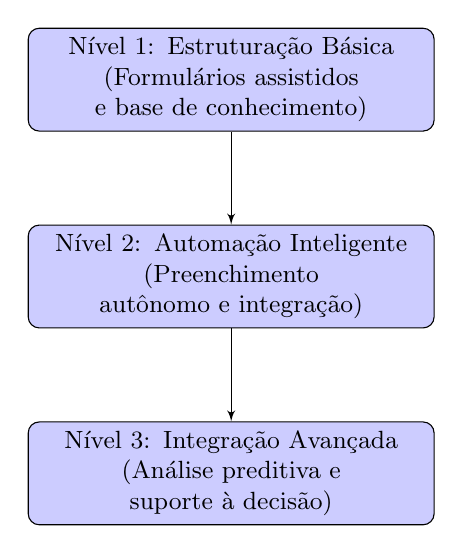
\begin{tikzpicture}[node distance=1.8cm, auto]
    % Definição dos estilos
    \tikzstyle{block} = [rectangle, draw, fill=blue!20, text width=14em, text centered, rounded corners, minimum height=3em, font=\small]
    \tikzstyle{line} = [draw, -latex']
    
    % Nós
    \node [block] (nivel1) {Nível 1: Estruturação Básica\\(Formulários assistidos e base de conhecimento)};
    \node [block, below of=nivel1, node distance=2.5cm] (nivel2) {Nível 2: Automação Inteligente\\(Preenchimento autônomo e integração)};
    \node [block, below of=nivel2, node distance=2.5cm] (nivel3) {Nível 3: Integração Avançada\\(Análise preditiva e suporte à decisão)};
    
    % Conexões
    \path [line] (nivel1) -- (nivel2);
    \path [line] (nivel2) -- (nivel3);
\end{tikzpicture}
\caption{Níveis de Implementação da Solução}
\end{figure}

\textbf{Componentes principais da solução:}

\begin{enumerate}
    \item \textbf{Interfaces de usuário:}
    \begin{itemize}
        \item Interface conversacional via WhatsApp: Canal principal de interação para maior acessibilidade
        \item Portal web responsivo: Interface alternativa com recursos visuais avançados
        \item Integração com SEI: Conexão com o sistema oficial de tramitação de processos
    \end{itemize}
    
    \item \textbf{Backend inteligente:}
    \begin{itemize}
        \item Motor de processamento de linguagem natural: Baseado em AWS Bedrock
        \item Base de conhecimento vetorial: Para busca semântica em documentos técnicos
        \item Sistema de formulários inteligentes: Com validação em tempo real e preenchimento assistido
        \item Orquestrador de processos: Para gestão de fluxos e integrações
    \end{itemize}
    
    \item \textbf{Repositório de conhecimento:}
    \begin{itemize}
        \item Documentação técnica: Normas, procedimentos, manuais e referências
        \item Templates de formulários: Modelos padronizados para diferentes tipos de solicitação
        \item Base de casos: Histórico de solicitações anteriores para referência e aprendizado
        \item FISPQ e documentação de produtos químicos: Catálogo digital de informações de segurança
    \end{itemize}
    
    \item \textbf{Módulos analíticos:}
    \begin{itemize}
        \item Dashboard de indicadores: Para monitoramento de KPIs
        \item Sistema de alertas: Para notificação proativa de prazos e pendências
        \item Módulo de relatórios: Para geração automática de relatórios gerenciais
        \item Análise de tendências: Para identificação preventiva de riscos
    \end{itemize}
\end{enumerate}

\textbf{Requisitos funcionais prioritários:}

\begin{itemize}
    \item Capacidade de interação em linguagem natural para orientar usuários
    \item Preenchimento assistido de formulários com validação em tempo real
    \item Consulta a base de conhecimento para responder dúvidas frequentes
    \item Integração com o SEI para submissão e acompanhamento de processos
    \item Notificação automática para equipe técnica e solicitantes
    \item Geração assistida de relatórios e documentos técnicos
    \item Gestão de documentos com versionamento e controle de acesso
    \item Análise e visualização de dados de segurança do trabalho
\end{itemize}

\textbf{Requisitos não-funcionais:}

\begin{itemize}
    \item Segurança: Proteção de dados sensíveis conforme LGPD
    \item Disponibilidade: Acesso 24/7 com pelo menos 99,5\% de uptime
    \item Desempenho: Tempo de resposta inferior a 2 segundos
    \item Escalabilidade: Capacidade para atender todos os campi do IFPE
    \item Usabilidade: Interface intuitiva para usuários com diferentes níveis de familiaridade tecnológica
    \item Manutenibilidade: Facilidade de atualização e expansão
    \item Interoperabilidade: Integração com sistemas existentes
\end{itemize}

\clearpage
\subsection{Estratégia de Implantação}

\subsubsection{Análise SWOT}

Para definir a estratégia mais adequada de implantação, realizamos uma análise SWOT (Forças, Fraquezas, Oportunidades e Ameaças) do projeto:

\begin{table}[h]
\centering
\begin{tcolorbox}[enhanced, colback=white, colframe=gray!40, arc=3mm, boxrule=0.5pt]
\scriptsize
\begin{tabular}{|p{7cm}|p{7cm}|}
\hline
\rowcolor{green!10}
\textbf{Forças (Strengths)} & \textbf{Fraquezas (Weaknesses)} \\
\hline
$\bullet$ Área de segurança bem regulamentada, facilitando a estruturação do conhecimento\\
$\bullet$ Especialista (César) engajado e conhecedor dos processos\\
$\bullet$ Apoio da alta administração do IFPE\\
$\bullet$ Processos relativamente estáveis e bem definidos\\
$\bullet$ Tecnologias de IA maduras disponíveis no mercado\\
$\bullet$ Equipe de projeto multidisciplinar
& 
$\bullet$ Recursos financeiros limitados da instituição pública\\
$\bullet$ Equipe técnica reduzida no setor de Segurança do Trabalho\\
$\bullet$ Resistência potencial à mudança de processos estabelecidos\\
$\bullet$ Dependência de infraestrutura de TI do IFPE\\
$\bullet$ Lacunas na documentação atual dos processos\\
$\bullet$ Complexidade de integração com sistemas legados (SEI) \\
\hline
\rowcolor{blue!10}
\textbf{Oportunidades (Opportunities)} & \textbf{Ameaças (Threats)} \\
\hline
$\bullet$ Crescente aceitação de interfaces conversacionais (chatbots)\\
$\bullet$ Possibilidade de expansão futura para outros domínios (saúde)\\
$\bullet$ Projeto piloto pode servir de modelo para outras instituições\\
$\bullet$ Evolução rápida das tecnologias de IA\\
$\bullet$ Potencial de publicações científicas sobre o projeto\\
$\bullet$ Melhoria da imagem institucional por inovação tecnológica
&
$\bullet$ Mudanças na gestão do IFPE podem afetar prioridades\\
$\bullet$ Restrições orçamentárias imprevistas\\
$\bullet$ Problemas de segurança de dados e conformidade com LGPD\\
$\bullet$ Dificuldades técnicas na integração com SEI\\
$\bullet$ Resistência cultural à adoção de IA no setor público\\
$\bullet$ Greves ou paralisações que afetem o cronograma\\
\hline
\end{tabular}
\end{tcolorbox}
\caption{Análise SWOT do Projeto}
\end{table}

\subsubsection{Estratégia selecionada}

Com base na análise SWOT e nas características do projeto, selecionamos uma estratégia de implantação \textbf{gradual e iterativa}, com as seguintes características:

\begin{enumerate}
    \item \textbf{Abordagem gradual em níveis:} Implementação em três níveis progressivos (Estruturação Básica, Automação Inteligente, Integração Avançada), conforme definido anteriormente.
    
    \item \textbf{Implantação por processos prioritários:} Início pelos processos mais críticos e de maior impacto, conforme identificado na matriz de processos suportados.
    
    \item \textbf{Programa piloto:} Seleção de um grupo inicial de usuários para validação antes da expansão para toda a instituição.
    
    \item \textbf{Ciclos de feedback contínuo:} Coleta e incorporação de feedback dos usuários ao longo de todo o processo.
    
    \item \textbf{Desenvolvimento ágil:} Utilização de metodologias ágeis para permitir ajustes e adaptações durante a implementação.
\end{enumerate}

\textbf{Justificativa da estratégia:}

Esta estratégia foi selecionada com base nos seguintes fatores identificados na análise SWOT:

\begin{itemize}
    \item \textbf{Mitigação de riscos:} A abordagem gradual permite identificar e corrigir problemas em estágios iniciais, sem comprometer todo o projeto.
    
    \item \textbf{Adaptação à cultura organizacional:} A implementação progressiva respeita o ritmo de adaptação da instituição, reduzindo a resistência à mudança.
    
    \item \textbf{Otimização de recursos limitados:} A priorização de processos críticos garante que os recursos sejam alocados para as áreas de maior impacto.
    
    \item \textbf{Aprendizado contínuo:} Os ciclos de feedback permitem o refinamento da solução com base na experiência real dos usuários.
    
    \item \textbf{Flexibilidade diante de incertezas:} A abordagem ágil proporciona flexibilidade para lidar com mudanças de contexto ou prioridades.
\end{itemize}

\subsubsection{Infraestrutura necessária}

A implementação do chatbot com IA para processos de segurança do trabalho requer a seguinte infraestrutura:

\begin{table}[H]
\centering
\begin{adjustbox}{max width=\textwidth}
\renewcommand{\arraystretch}{1.2}
\begin{tabular}{|p{3cm}|p{5cm}|p{4cm}|p{3cm}|}
\hline
\rowcolor{gray!20}
\textbf{Categoria} & \textbf{Recursos} & \textbf{Especificações} & \textbf{Fase Necessária} \\
\hline
\multirow{3}{*}{Servidores} & Ambiente de Desenvolvimento & Servidor virtual com 8 vCPUs, 16GB RAM, 100GB SSD & Preparação \\
\cline{2-4}
 & Ambiente de Homologação & Servidor virtual com 8 vCPUs, 16GB RAM, 100GB SSD & Piloto \\
\cline{2-4}
 & Ambiente de Produção & Servidor virtual com 16 vCPUs, 32GB RAM, 500GB SSD & Expansão \\
\hline
\multirow{3}{*}{Serviços em Nuvem} & AWS Bedrock & API para modelos de IA como Claude Opus & Todas \\
\cline{2-4}
 & Amazon S3 & Armazenamento de documentos e artefatos & Todas \\
\cline{2-4}
 & Amazon RDS & Banco de dados relacional & Todas \\
\hline
\multirow{2}{*}{Canais de Comunicação} & API WhatsApp Business & Licença para envio de mensagens em volume & Piloto em diante \\
\cline{2-4}
 & Domínio e SSL & Certificados para portal web & Preparação \\
\hline
\multirow{2}{*}{Segurança} & Soluções de Backup & Backup diário com retenção de 30 dias & Todas \\
\cline{2-4}
 & Ferramentas de Monitoramento & Sistema de logs e alertas & Todas \\
\hline
\multirow{2}{*}{Desenvolvimento} & Ambientes de Desenvolvimento & Acesso aos ambientes e ferramentas de desenvolvimento & Preparação \\
\cline{2-4}
 & Repositório de Código & Sistema de controle de versão (Git) & Preparação \\
\hline
\end{tabular}
\end{adjustbox}
\caption{Infraestrutura Necessária para Implantação}
\end{table}

\subsubsection{Metodologia de trabalho}

Para garantir uma implementação bem-sucedida, adotaremos a seguinte metodologia de trabalho:

\begin{enumerate}
    \item \textbf{Gestão de projeto:} Utilização do framework Scrum adaptado, com sprints de duas semanas e reuniões diárias de sincronização.
    
    \item \textbf{Monitoramento de progresso:} Utilização de quadro Kanban para visualização do fluxo de trabalho e acompanhamento de tarefas.
    
    \item \textbf{Reuniões regulares:}
    \begin{itemize}
        \item Reuniões diárias (15 minutos): Sincronização da equipe de desenvolvimento
        \item Reuniões semanais (1 hora): Acompanhamento com stakeholders principais
        \item Reuniões quinzenais (2 horas): Demonstração de incrementos e coleta de feedback
        \item Reuniões mensais (3 horas): Revisão de progresso e planejamento estratégico
    \end{itemize}
    
    \item \textbf{Documentação:}
    \begin{itemize}
        \item Backlog do produto: Lista priorizada de requisitos e funcionalidades
        \item Documentação técnica: Arquitetura, integrações e configurações
        \item Atas de reunião: Registro das decisões e próximos passos
        \item Relatórios de progresso: Status do projeto, riscos e planos de mitigação
    \end{itemize}
    
    \item \textbf{Comunicação:}
    \begin{itemize}
        \item E-mail corporativo: Para comunicações formais e documentação
        \item Grupo de mensagens instantâneas: Para comunicação rápida e alinhamentos
        \item Reuniões virtuais: Para discussões e demonstrações
        \item Portal do projeto: Para compartilhamento de artefatos e acompanhamento
    \end{itemize}
    
    \item \textbf{Validação e testes:}
    \begin{itemize}
        \item Testes unitários: Validação de componentes individuais
        \item Testes de integração: Verificação da interação entre componentes
        \item Testes de usuário: Validação da experiência do usuário com cenários reais
        \item Homologação: Aprovação formal pelos stakeholders
    \end{itemize}
\end{enumerate}

\clearpage
\subsection{Dimensionamento e Perfil da Equipe para a Implantação da Melhoria}

A implantação do chatbot com IA para processos de segurança do trabalho requer uma equipe multidisciplinar com diferentes competências. A seguir, detalhamos o dimensionamento e o perfil necessários:

\begin{table}[H]
\centering
\begin{adjustbox}{max width=\textwidth}
\renewcommand{\arraystretch}{1.2}
\begin{tabular}{|p{3cm}|p{3cm}|p{3cm}|p{6cm}|}
\hline
\rowcolor{gray!20}
\textbf{Papel} & \textbf{Quantidade} & \textbf{Dedicação} & \textbf{Responsabilidades} \\
\hline
Gerente de Projeto & 1 & 100\% & Coordenação geral, gestão de recursos, comunicação com stakeholders, gerenciamento de riscos \\
\hline
Arquiteto de Soluções & 1 & 50\% & Definição da arquitetura técnica, seleção de tecnologias, planejamento de integrações \\
\hline
Especialista em IA & 1 & 50\% & Treinamento de modelos, configuração de APIs de IA, otimização de desempenho \\
\hline
Desenvolvedor Full Stack & 2 & 100\% & Desenvolvimento de front-end, back-end e integrações \\
\hline
Engenheiro de Dados & 1 & 50\% & Modelagem de dados, ETL, estruturação da base de conhecimento \\
\hline
Designer UX/UI & 1 & 50\% & Design de interfaces, jornadas de usuário, testes de usabilidade \\
\hline
Especialista em Segurança & 1 & 30\% & Implementação de controles de segurança, conformidade com LGPD \\
\hline
Analista de Qualidade & 1 & 50\% & Testes, validação de requisitos, garantia de qualidade \\
\hline
Especialista em Segurança do Trabalho & 1 & 30\% & Validação técnica, fornecimento de conteúdo, homologação funcional \\
\hline
Analista de Negócios & 1 & 50\% & Levantamento de requisitos, modelagem de processos, interface com usuários \\
\hline
\end{tabular}
\end{adjustbox}
\caption{Dimensionamento e Perfil da Equipe}
\end{table}

\subsection{Custos Associados à Implantação da Melhoria}

A estimativa de custos para a implantação do chatbot com IA para processos de segurança do trabalho foi calculada considerando os recursos humanos, infraestrutura, licenças e serviços necessários:

\begin{table}[h]
\centering
\begin{tcolorbox}[enhanced, colback=white, colframe=gray!40, arc=3mm, boxrule=0.5pt]
\scriptsize
\begin{tabular}{|p{2.8cm}|p{3.2cm}|r|r|}
\hline
\rowcolor{gray!20}
\textbf{Categoria} & \textbf{Item} & \textbf{Valor Mensal (R\$)} & \textbf{Valor Total (R\$)} \\
\hline
\multirow{5}{*}{Recursos Humanos} & Equipe interna (dedicação parcial) & 12.000,00 & 144.000,00 \\
\cline{2-4}
 & Consultoria especializada em IA & 15.000,00 & 45.000,00 (3 meses) \\
\cline{2-4}
 & Desenvolvimento terceirizado & 25.000,00 & 125.000,00 (5 meses) \\
\cline{2-4}
 & Suporte técnico pós-implantação & 8.000,00 & 48.000,00 (6 meses) \\
\cline{2-4}
 & \textbf{Subtotal RH} & & \textbf{362.000,00} \\
\hline
\multirow{4}{*}{\parbox{2.8cm}{Infraestrutura\\ e Serviços}} & Servidores em nuvem & 3.500,00 & 42.000,00 \\
\cline{2-4}
 & Serviços AWS (Bedrock, S3, RDS) & 5.500,00 & 66.000,00 \\
\cline{2-4}
 & API WhatsApp Business & 1.800,00 & 21.600,00 \\
\cline{2-4}
 & \textbf{Subtotal Infraestrutura} & & \textbf{129.600,00} \\
\hline
\multirow{3}{*}{\parbox{2.8cm}{Licenças e\\ Ferramentas}} & Ferramentas de desenvolvimento & - & 10.000,00 (único) \\
\cline{2-4}
 & Licenças de software & 1.500,00 & 18.000,00 \\
\cline{2-4}
 & \textbf{Subtotal Licenças} & & \textbf{28.000,00} \\
\hline
\multirow{4}{*}{Outros Custos} & Treinamento de usuários & - & 18.000,00 (único) \\
\cline{2-4}
 & Documentação e materiais & - & 8.000,00 (único) \\
\cline{2-4}
 & Contingência (15\%) & - & 81.840,00 \\
\cline{2-4}
 & \textbf{Subtotal Outros} & & \textbf{107.840,00} \\
\hline
\multicolumn{2}{|r|}{\textbf{TOTAL}} & & \textbf{627.440,00} \\
\hline
\end{tabular}
\end{tcolorbox}
\caption{Custos Associados à Implantação}
\end{table}

\textbf{Observações sobre os custos:}

\begin{itemize}
    \item A estimativa foi otimizada para um horizonte de 10 meses, incluindo as mesmas fases de preparação, piloto, expansão e consolidação, porém com maior eficiência.
    \item Utilizaremos recursos internos de forma mais intensiva, resultando em menor dependência de consultoria externa.
    \item A abordagem em nuvem foi renegociada para obter descontos significativos de volume e compromisso anual.
    \item A estratégia de desenvolvimento foi redesenhada para utilizar componentes reutilizáveis e frameworks open-source.
    \item A redução de 31\% no orçamento total (de R\$ 908.500,00 para R\$ 627.440,00) foi obtida sem comprometer os objetivos centrais do projeto.
\end{itemize}

\subsection{Cronograma Macro}

O cronograma macro para a implantação do chatbot com IA para processos de segurança do trabalho está organizado em quatro fases principais, com duração total de 22 semanas:

\begin{table}[h]
\centering
\begin{tcolorbox}[enhanced, colback=white, colframe=gray!40, arc=3mm, boxrule=0.5pt]
\scriptsize
\begin{tabular}{|p{1.8cm}|p{1cm}|p{4.8cm}|p{4cm}|}
\hline
\rowcolor{gray!20}
\textbf{Fase} & \textbf{Duração} & \textbf{Principais Atividades} & \textbf{Entregas} \\
\hline
\multirow{4}{*}{Preparação} & \multirow{4}{*}{4 semanas} & $\bullet$ Definição detalhada de requisitos & $\bullet$ Documento de requisitos aprovado \\
\cline{3-4}
 & & $\bullet$ Configuração da infraestrutura & $\bullet$ Ambientes configurados \\
\cline{3-4}
 & & $\bullet$ Treinamento inicial da IA & $\bullet$ Base de conhecimento inicial \\
\cline{3-4}
 & & $\bullet$ Definição de métricas & $\bullet$ Framework de avaliação \\
\hline
\multirow{4}{*}{Piloto} & \multirow{4}{*}{6 semanas} & $\bullet$ Desenvolvimento do Nível 1 & $\bullet$ Chatbot básico funcional \\
\cline{3-4}
 & & $\bullet$ Seleção e treinamento de usuários piloto & $\bullet$ Grupo piloto treinado \\
\cline{3-4}
 & & $\bullet$ Teste com grupo piloto & $\bullet$ Relatório de feedback \\
\cline{3-4}
 & & $\bullet$ Ajustes baseados no feedback & $\bullet$ Versão refinada do Nível 1 \\
\hline
\multirow{4}{*}{Expansão} & \multirow{4}{*}{8 semanas} & $\bullet$ Desenvolvimento do Nível 2 & $\bullet$ Funcionalidades de automação \\
\cline{3-4}
 & & $\bullet$ Treinamento de multiplicadores & $\bullet$ Equipe de multiplicadores formada \\
\cline{3-4}
 & & $\bullet$ Implantação em departamentos selecionados & $\bullet$ Solução disponível para áreas selecionadas \\
\cline{3-4}
 & & $\bullet$ Integração com sistemas existentes & $\bullet$ Conectores funcionais com SEI \\
\hline
\multirow{4}{*}{Consolidação} & \multirow{4}{*}{4 semanas} & $\bullet$ Desenvolvimento de recursos do Nível 3 & $\bullet$ Funcionalidades avançadas \\
\cline{3-4}
 & & $\bullet$ Implantação geral & $\bullet$ Solução disponível para toda instituição \\
\cline{3-4}
 & & $\bullet$ Avaliação de resultados & $\bullet$ Relatório de desempenho \\
\cline{3-4}
 & & $\bullet$ Planejamento de melhorias contínuas & $\bullet$ Roadmap de evolução \\
\hline
\end{tabular}
\end{tcolorbox}
\caption{Cronograma Macro de Implantação}
\end{table}

\begin{figure}[h]
\centering
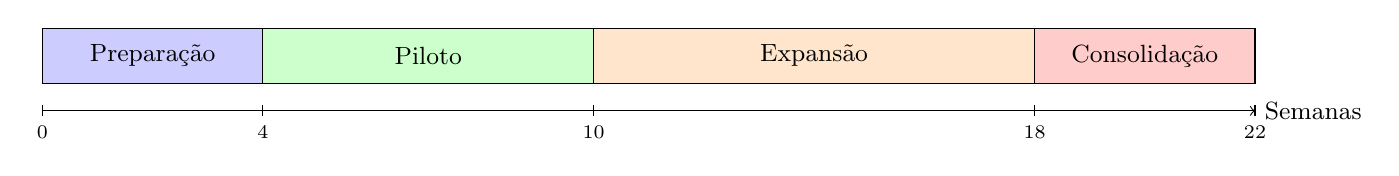
\begin{tikzpicture}[scale=0.7]
\draw[->] (0,0) -- (22,0) node[right] {\small Semanas};
\foreach \x in {0,4,10,18,22}
    \draw (\x,0.1) -- (\x,-0.1) node[below] {\scriptsize \x};

\filldraw[fill=blue!20] (0,0.5) rectangle (4,1.5) node[midway, font=\small] {Preparação};
\filldraw[fill=green!20] (4,0.5) rectangle (10,1.5) node[midway, font=\small] {Piloto};
\filldraw[fill=orange!20] (10,0.5) rectangle (18,1.5) node[midway, font=\small] {Expansão};
\filldraw[fill=red!20] (18,0.5) rectangle (22,1.5) node[midway, font=\small] {Consolidação};
\end{tikzpicture}
\caption{Linha do Tempo do Projeto}
\end{figure}

\clearpage
\subsection{Plano de medições e análise}

Para avaliar o sucesso da implantação e os benefícios entregues pela solução, estabelecemos um conjunto de indicadores-chave de desempenho (KPIs) que serão monitorados ao longo do projeto:

\subsubsection{Indicador: Tempo médio de preenchimento de formulários}

\textbf{Finalidade:} Avaliar a eficiência da solução na redução do tempo necessário para preencher formulários relacionados à segurança do trabalho.

\textbf{Como medir:} 
\begin{itemize}
    \item Linha base: Medição do tempo médio atual através de observação direta e entrevistas (estimado em 45 minutos)
    \item Pós-implantação: Registro automático do tempo entre início e conclusão do preenchimento via chatbot
    \item Frequência: Mensal
\end{itemize}

\textbf{Análise de impacto:} A redução do tempo de preenchimento tem impacto direto na produtividade dos servidores e na agilidade dos processos. A meta é reduzir em 67\% (para 15 minutos) em 12 meses.

\subsubsection{Indicador: Taxa de preenchimento correto na primeira tentativa}

\textbf{Finalidade:} Avaliar a eficácia da solução na redução de erros e retrabalho.

\textbf{Como medir:} 
\begin{itemize}
    \item Linha base: Percentual de formulários que precisam ser corrigidos ou complementados (estimado em 40\% de acerto)
    \item Pós-implantação: Registro automático de formulários completos e válidos na primeira submissão
    \item Frequência: Mensal
\end{itemize}

\textbf{Análise de impacto:} O aumento da taxa de acerto reduz retrabalho tanto para solicitantes quanto para a equipe técnica. A meta é aumentar para 80\% em 12 meses.

\subsubsection{Indicador: Consultas básicas direcionadas à equipe técnica}

\textbf{Finalidade:} Avaliar o grau de desoneração da equipe técnica de atividades de baixo valor agregado.

\textbf{Como medir:} 
\begin{itemize}
    \item Linha base: Contagem de consultas básicas semanais recebidas pela equipe técnica (estimado em 35)
    \item Pós-implantação: Registro de consultas não resolvidas pelo chatbot
    \item Frequência: Semanal
\end{itemize}

\textbf{Análise de impacto:} A redução de consultas básicas permite que a equipe técnica se concentre em atividades que exigem expertise especializada. A meta é reduzir para 8 consultas semanais em 12 meses.

\subsubsection{Indicador: Dúvidas atendidas sem intervenção humana}

\textbf{Finalidade:} Avaliar a autonomia e eficácia do chatbot.

\textbf{Como medir:} 
\begin{itemize}
    \item Linha base: Percentual de dúvidas que podem ser resolvidas automaticamente (estimado em 20\%)
    \item Pós-implantação: Percentual de consultas resolvidas pelo chatbot sem escalação
    \item Frequência: Mensal
\end{itemize}

\textbf{Análise de impacto:} O aumento da resolução automática amplia a disponibilidade do serviço e reduz dependência de recursos humanos limitados. A meta é aumentar para 80\% em 12 meses.

\subsubsection{Indicador: Satisfação do usuário}

\textbf{Finalidade:} Avaliar a percepção dos usuários sobre a qualidade e utilidade da solução.

\textbf{Como medir:} 
\begin{itemize}
    \item Linha base: Pesquisa de satisfação com serviços atuais (estimado em 65\%)
    \item Pós-implantação: Pesquisa de satisfação e feedback pós-interação com chatbot
    \item Frequência: Trimestral
\end{itemize}

\textbf{Análise de impacto:} A satisfação do usuário está diretamente relacionada à adoção e ao sucesso da solução. A meta é aumentar para 90\% em 12 meses.

\subsubsection{Indicador: Tempo de resposta para solicitações}

\textbf{Finalidade:} Avaliar a agilidade no atendimento às solicitações.

\textbf{Como medir:} 
\begin{itemize}
    \item Linha base: Tempo médio entre solicitação e resposta final (estimado em 48 horas)
    \item Pós-implantação: Registro automático do ciclo completo de solicitação
    \item Frequência: Mensal
\end{itemize}

\textbf{Análise de impacto:} A redução do tempo de resposta melhora a experiência do usuário e a eficiência operacional. A meta é reduzir para 12 horas em 12 meses.

\subsubsection{Indicador: Volume de documentação digital vs. papel}

\textbf{Finalidade:} Avaliar o grau de digitalização dos processos.

\textbf{Como medir:} 
\begin{itemize}
    \item Linha base: Percentual de documentos em formato digital (estimado em 40\%)
    \item Pós-implantação: Proporção entre documentos digitais e físicos
    \item Frequência: Trimestral
\end{itemize}

\textbf{Análise de impacto:} O aumento da digitalização facilita o acesso, reduz custos e melhora a gestão documental. A meta é aumentar para 95\% em 12 meses.

\clearpage
\section{Conclusões e Considerações Finais}

A implantação do chatbot com IA para processos de segurança do trabalho representa uma oportunidade significativa para transformar e modernizar os serviços prestados pelo setor de Segurança do Trabalho do SIASS/IFPE. Este plano de implantação foi elaborado com base em uma análise detalhada do contexto atual, identificação de desafios e oportunidades, e definição de uma estratégia gradual e iterativa para maximizar as chances de sucesso.

Os principais benefícios esperados com a implementação desta solução incluem:

\begin{itemize}
    \item \textbf{Eficiência operacional:} Redução significativa no tempo de processamento de solicitações e no esforço administrativo da equipe técnica.
    
    \item \textbf{Padronização e qualidade:} Maior consistência nos processos e documentos, com redução de erros e retrabalho.
    
    \item \textbf{Acessibilidade:} Disponibilização de informações e serviços de forma mais acessível e intuitiva para todos os servidores.
    
    \item \textbf{Preservação do conhecimento:} Estruturação e centralização do conhecimento técnico em segurança do trabalho.
    
    \item \textbf{Inteligência organizacional:} Geração de dados e insights para tomada de decisão baseada em evidências.
    
    \item \textbf{Evolução tecnológica:} Posicionamento do IFPE como instituição inovadora na aplicação de tecnologias avançadas para melhoria de serviços.
\end{itemize}

Para garantir o sucesso desta iniciativa, algumas considerações importantes devem ser observadas:

\begin{enumerate}
    \item \textbf{Gestão da mudança:} É fundamental investir em comunicação, treinamento e envolvimento dos usuários desde as fases iniciais do projeto.
    
    \item \textbf{Flexibilidade:} O plano deve ser adaptável para acomodar aprendizados e necessidades emergentes ao longo da implementação.
    
    \item \textbf{Foco no valor:} As decisões devem sempre priorizar o valor entregue aos usuários e à instituição, não apenas aspectos técnicos.
    
    \item \textbf{Visão de longo prazo:} Embora implementado em fases, o projeto deve manter alinhamento com a visão estratégica de longo prazo.
    
    \item \textbf{Sustentabilidade:} A solução deve ser projetada para ser mantida e evoluída após a conclusão do projeto inicial.
\end{enumerate}

A estratégia de implementação em três níveis progressivos permite uma abordagem controlada e sustentável, minimizando riscos e maximizando o aprendizado. Iniciando com funcionalidades básicas de preenchimento assistido de formulários e base de conhecimento, evoluindo para automação inteligente e integração de sistemas, e finalmente alcançando recursos avançados de análise preditiva e suporte à decisão, o projeto oferece entregas de valor em cada etapa.

O sucesso desta iniciativa não depende apenas de aspectos tecnológicos, mas principalmente do engajamento das pessoas e da capacidade de integrar a solução aos processos e à cultura da instituição. O comprometimento da alta administração, a participação ativa dos especialistas em segurança do trabalho e a adoção pelos usuários finais são fatores críticos para que os benefícios esperados sejam plenamente alcançados.

Recomenda-se o início imediato da fase de preparação, seguindo o cronograma e a metodologia definidos neste plano, com acompanhamento regular dos indicadores estabelecidos para avaliar o progresso e o impacto da solução.

\clearpage
\thispagestyle{empty}
\section*{Folha de Assinaturas}

\vspace{2cm}

\centering
\begin{tabular}{p{7cm}p{7cm}}
\line(1,0){200} & \line(1,0){200} \\
\centering Pedro Henrique Souza Balbino & \centering Marco Antônio Eugênio Araujo \\
\centering Gerente de Projeto & \centering Cliente/Representante SIASS \\
\\[1cm]
\line(1,0){200} & \line(1,0){200} \\
\centering Eric Bezerra Londres Barreto & \centering Mauro César de Oliveira \\
\centering Arquiteto de Soluções & \centering Especialista em Segurança do Trabalho \\
\\[1cm]
\line(1,0){200} & \line(1,0){200} \\
\centering Sara Simone Emilay de Araujo Pereira & \centering Luis Felipe Guedes Souto Moreira \\
\centering Analista de Negócios & \centering Desenvolvedor \\
\end{tabular}

\vfill
\begin{center}
\large
Recife, Abril de 2025
\end{center}

\end{document}